% Description, implementation, alignment corrections, performance and latency

\subsubsection{The pre-trigger from the pad towers}

The sTGC trigger is based on determining track coordinates from the centroids of strip charges.
Transmitting $\approx$280,000 strip charges off-detector would requires bandwidths not practical for today's optical interconnect technology.
To reduce the amount of data sent to the off-detector Trigger Processors,
the sTGC uses an 8-fold coincidence along detector pads towers to identify regions where a possible muon candidate has passed.
See Figure\,\ref{fig:LL_PadSelect} and Ref.\cite{padTower}.
Information only from sTGC strips passing through the tower selected by the Pad Trigger is transmitted off-detector to the Trigger Processor.

\begin{figure}[h]
  \centering
  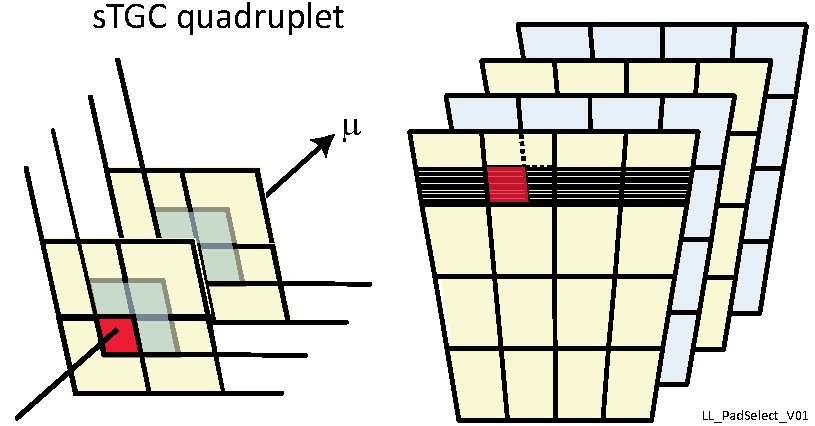
\includegraphics[width=0.55\textwidth]{figures/LL_PadSelect_V01.pdf}
  \caption{The Pad Trigger selects the strips passing through a pad tower made from a coincidence of overlapping pads. One layer of the selected strips is shown.}
  \label{fig:LL_PadSelect}
\end{figure}

It is expected that sometimes a layer of strips will not be useable because its cluster of strips is very wide
due to a $\delta$-ray or neutron, or its signals are saturated due to a neutron track, or the detector layer has become defective.
The algorithm described below discards such clusters and defective layers.
There are enough layers that precise centroids can none-the-less be calculated with less than the full four layers of a quadruplet.

An important parameter is the number of track segments expected to be found,
given the rate of background tracks that successfully pass through all layers of the NSW and could trigger the Pad Trigger.
An estimate of the probability of 1, 2, and 3~segments in a sector is shown in Figure\,\ref{fig:DL_segRates}.
See Ref.~\cite{LellouchRates} for details of the calculation and assumptions.
The planned sTGC trigger path supports transfer of the strip data for up to four track segments.
The figure shows that the losses from this limit are negligible.

\begin{figure}[h]
\centering
   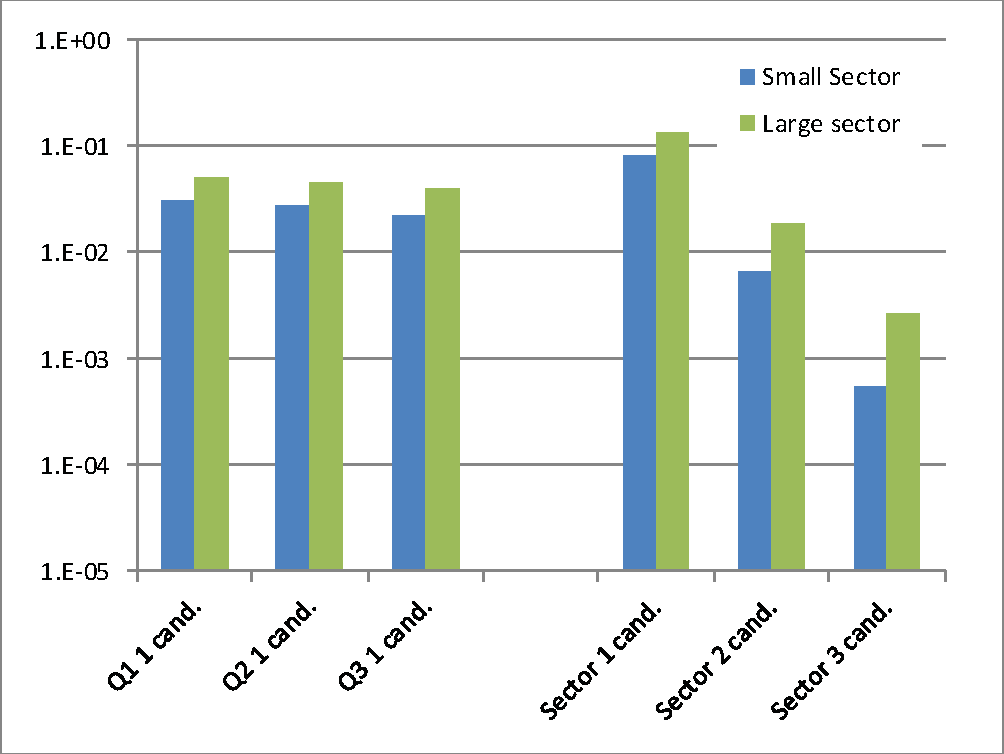
\includegraphics[width=.55\textwidth]{figures/DL_segRates_V01.pdf}
   \caption{Left: The fraction of BCs with one segment (candidate) for each of the three quadruplets.
           Right: The fraction of BCs with one, two, and three segments in a sector. From Ref.~\cite{LellouchRates}}
   \label{fig:DL_segRates}
\end{figure}

\subsubsection{Finding track segments and calculating their parameters}

The sTGC algorithm calculates the $\Delta\theta$, $\phi$ index and R\,index of a track segment.
The algorithm input is an active band of strips for each of the 8~layers.
The information of a band consists of 17~strip ``charges'' measured by the 6-bit flash ADC in the VMM front end ASIC.
The 17~strips include 13~strips of the band itself plus two strips from each of neighboring bands
that provide for charge spreading to adjacent bands.
First, the centroid for each of 8 layers is calculated using the FPGA's built-in DSP (Digital Signal Processing) blocks.
Figure\,\ref{fig:JN_CENTROID_algorithm} shows the centroid calculation algorithm for a single layer.

\begin{figure}[h]
   \centering
   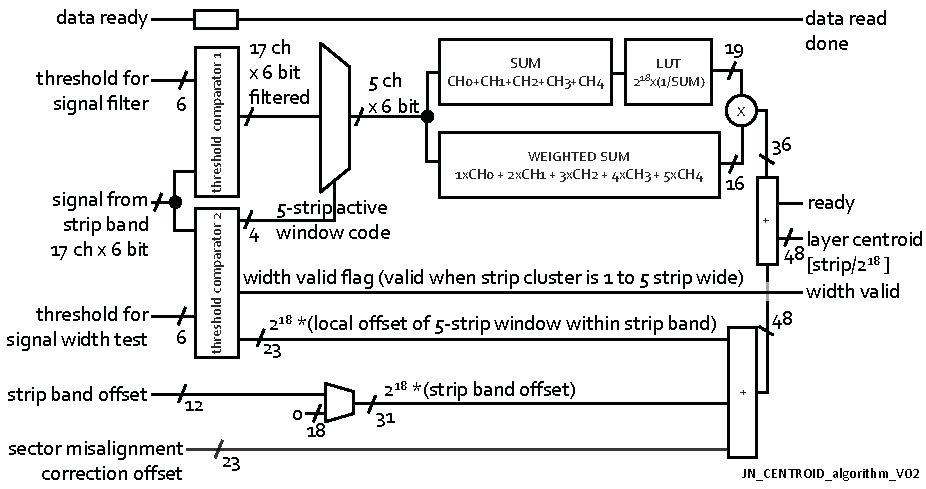
\includegraphics[width=0.9\textwidth]{figures/JN_CENTROID_algorithm_V02.pdf}
   \caption{The centroid algorithm for a single layer, total latency of 8 clocks (320\,MHz)}
   \label{fig:JN_CENTROID_algorithm}
\end{figure}

\FloatBarrier   %%%% recheck need

\vspace{8mm}

Two separate configurable thresholds are provided, one for filtering the input strip signal
and another for defining the signal width in number of strips.
A valid strip band is defined as a band that has one to five active strips,
in all other cases the layer centroid calculation result will have a ``width valid'' flag set to zero.
When ``width valid'' flag of a layer is zero, this layer does not participate in further calculations.

A local center of mass is calculated from the five values in the 5-strip window.
The calculation formula is a weighted mean:
$\frac{\sum_{n=1}^{5} n \times Q_n}{\sum_{n=1}^{5} Q_n}$.
The band's global offset comes from the band-id, i.e.\,the row index of the active pad tower,
and is added to the local-to-band calculation result. Layer centroid calculation algorithm's latency is 8~clocks (320\,MHz).

For both of the 4-layer quadruplets, a centroid is calculated as an average of its valid layer centroids.
This is shown on Figure\,\ref{fig:JN_QCENTROID_algorithm}. Quadruplet centroid calculation latency is 3~clocks (320\,MHz).

\begin{figure}[h]
   \centering
   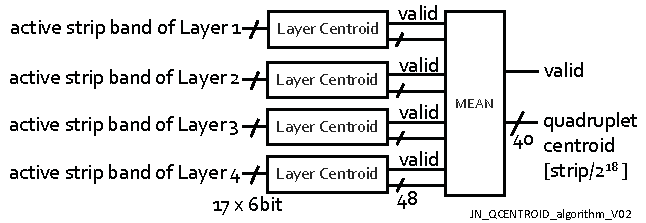
\includegraphics[width=0.72\textwidth]{figures/JN_QCENTROID_algorithm_V02.pdf}
   \caption{Calculation of the quadruplet centroid, total latency of 11 clocks (320\,MHz)}
   \label{fig:JN_QCENTROID_algorithm}
\end{figure}

%\clearpage
It is possible that during the algorithm execution it is found that there is only one valid quadruplet centroid (i.e.\ it has at least one valid layer centroid).
This situation occurs, for example, when the track passes through the frame of one of the quadruplets.
In this case we use the coordinates within this valid quadruplet to calculate a $\Delta\theta$, albeit with much poorer accuracy.
In order that the algorithm have the same latency in either case,
the low quality result for each of the quadruplets is calculated in parallel to the main algorithm.
If the main algorithm, fails one of the low quality results maybe used instead.

Having the pivot quadruplet centroid value allows the algorithm to define a range for the valid values of the confirmation quadruplet centroid.
A valid range for the confirmation quadruplet centroid value is defined by the maximum deviation of $\pm$15\,mrad from the infinite momentum track angle
as shown in Figure\,\ref{fig:JN_DeltaTheta}.
The maximum allowed deviation, $\Delta\theta_{cut}$, is configurable.

\begin{figure}[h]
   \centering
   \includegraphics[width=0.97\textwidth]{figures/JN_DeltaTheta_V02.pdf}
   \caption{Definition of the valid range of the confirmation quadruplet centroid values, i.e.\ within $\Delta\theta_{cut}$}
   \label{fig:JN_DeltaTheta}
\end{figure}

The $\Delta\theta$ margins LUT defines valid RB (quadruplet B centroid) value ranges for each possible RA (quadruplet A centroid) value.
Each range maps RB onto one of the valid values of $\Delta\theta$; out-of-range values of RB are marked by setting ``valid'' flag to zero.
Figure\,\ref{fig:JN_DeltaThetaBlk} shows a block diagram of the $\Delta\theta$ calculation path.

\begin{figure}[h]
   \centering
   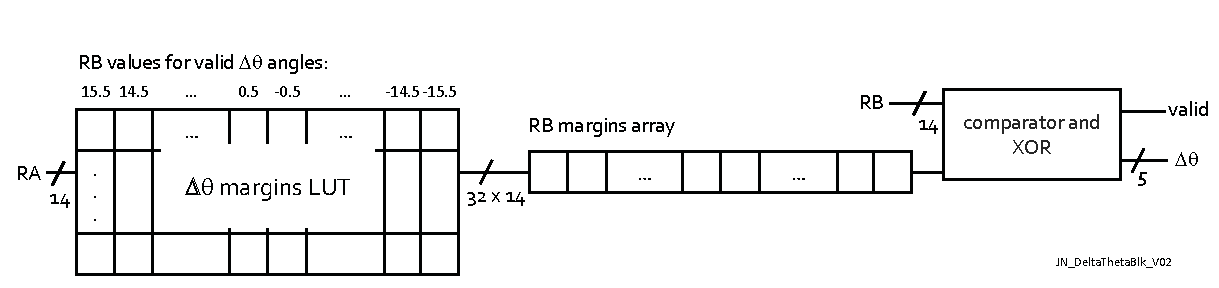
\includegraphics[width=0.95\textwidth]{figures/JN_DeltaThetaBlk_V02.pdf}
   \caption{The Look-up-Table scheme for producing $\Delta\theta$ within the desired cut}
   \label{fig:JN_DeltaThetaBlk}
\end{figure}


R index is a trajectory projection on a Big Wheel and is calculated directly from RA and RB values using mapping conversion LUTs,
as shown on Figure\,\ref{fig:JN_RindexCalcBlk}. Calculation of $\Delta\theta$ and R index is done in parallel with latency of 3 clocks (320\,MHz).



\begin{figure}[h]
   \centering
   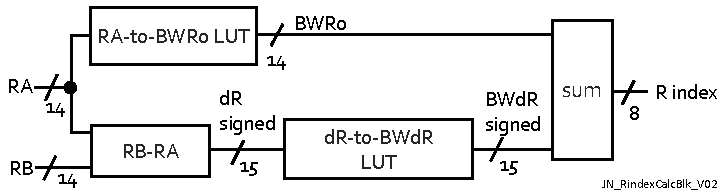
\includegraphics[width=0.75\textwidth]{figures/JN_RindexCalcBlk_V02.pdf}
   \caption{Calculation of the R\,index}
   \label{fig:JN_RindexCalcBlk}
\end{figure}

\vspace{-3mm}
\paragraph{Latency and FPGA resources needed}
The total latency for the sTGC algorithm is 18 320\,MHz clocks, including 14 for the algorithm itself plus four more for preparation of inputs and outputs.
One segment finder consumes 1.2\% of the FPGA Virtex\,7~690T LUT resources, 9\% of the Block RAMs and 1.8\% of the DSPs.
This allows ample resources to add two single quadruplet segment finders and the misalignment correction calculator, all replicated four times.
The ancillary functions must also be added.

%\begin{figure}[h]
%   \centering
%   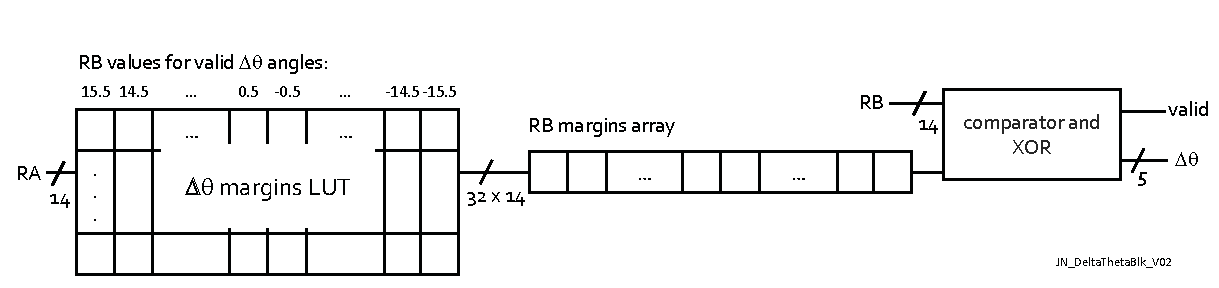
\includegraphics[width=0.97\textwidth]{figures/JN_DeltaThetaBlk_V02.pdf}
%   \caption{The Look-up-Table scheme for producing $\Delta\theta$ within the desired cut}
%   \label{fig:JN_DeltaThetaBlk}
%\end{figure}
%
%
%\begin{figure}[h]
%   \centering
%   \includegraphics[width=0.97\textwidth]{figures/JN_RindexCalc_V02.pdf}
%   \caption{Calculation of the R\,index}
%   \label{fig:JN_RindexCalc}
%\end{figure}

\FloatBarrier

\subsubsection{Compensating for misalignments}

The sTGC algorithm provides quadruplet misalignment correction for the cases that are shown in Figure\,\ref{fig:DL_misalignment}:
\begin{enumerate}\itemsep-6pt
\item[(1)] displacement along r-axis (axis orthogonal to the beam axis),
\item[(2)] displacement along the z-axis (beam axis),
\item[(3)] rotational displacement around the detector edge orthogonal to the r-axis,
\item[(4)] rotational displacement around the r-axis
\item[(5)] rotational displacement around the axis parallel to the z-axis.
\end{enumerate}

\begin{figure}[h]
   \centering
   \includegraphics[width=0.2\textwidth]{figures/DL_misalignment_V01.pdf}
   \caption{The possible misalignments of a sTGC quadruplet}
   \label{fig:DL_misalignment}
\end{figure}

Each of the six quadruplets of a sector are divided into sections by band-ID and $\phi$-ID.
For each of these sections, four constant geometrical parameters ($dr$, $dr^{2}$, $dr d\phi$, $d\phi$) are stored in six 2-D look-up tables.
Each cell of the LUT contains a set of the four values for each combination of band-ID
(or predefined contiguous set of band IDs) and $\phi$-ID (or predefined contiguous set of $\phi$-IDs).
Five measured mechanical alignment values for each of six quadruplets of a sector are stored in a RAM and updated by the calibration process.
The total correction offset for one quadruplet is calculated as a dot product of the two entries.
This misalignment calculation, as shown on Figure\,\ref{fig:JN_misalignment_correction},
is done in parallel with the layer centroid algorithm and is added to its result, i.e.\ one additional (320\,MHz) clock latency.

\begin{figure}[h]
   \centering
   \includegraphics[width=0.9\textwidth]{figures/JN_misalignment_correction_V02.pdf}
   \caption{LUT-based misalignment correction algorithm. Numbers in orange represent the possible chamber misalignment cases according to Figure\,\ref{fig:DL_misalignment}.}
   \label{fig:JN_misalignment_correction}
\end{figure}

\FloatBarrier


